\documentclass[12pt,letterpaper]{article}


\newcommand{\studentname}{Ben Bassett}

\title{\textsc{Lab 11: Newton’s Ring(s) of Power}}
\newcommand{\shorttitle}{Newton’s Rings}

\newcommand{\course}{PHY310}
\newcommand{\labdate}{11-19-2024}

%------------------------------------------------------------------------------------------------------------

\usepackage[letterpaper,left=1in,right=1in,bottom=1in,top=1in]{geometry}
\usepackage{fancyhdr}
\usepackage{subfigure}
\usepackage{graphicx}
\usepackage{amsmath}
\DeclareMathOperator{\sinc}{sinc}
\usepackage{cleveref}
\usepackage{booktabs}
\usepackage[british]{babel}
\usepackage[square,comma,numbers,sort&compress]{natbib}
\usepackage{csvsimple}
\usepackage{graphicx}
\usepackage{pgfplotstable}
\usepackage{textcomp,gensymb}
\usepackage{array}
\usepackage{tabu}
\usepackage{multirow}
\usepackage{url}
\usepackage{lipsum}
\usepackage{dsfont}
\usepackage{fontspec}
\pgfplotsset{compat=1.9}% supress warning
\begin{document}

%------------------------------------------------------------------------------------------------------------

\setlength{\parindent}{1em}
\setlength{\parskip}{0.5em}
\author{\course~Lab Journal \\ \\ \studentname} % \,\& \labpartner}
\date{\labdate}

% \setmainfont{Wingdings-Regular.ttf}


\renewcommand\abstractname{Summary}

\pagestyle{fancy}
\fancyhead{}
\fancyhead[l]{\course:~\shorttitle}
\fancyhead[r]{\studentname}
\fancyfoot{}
\fancyfoot[C]{\thepage}
\renewcommand{\headrulewidth}{0pt}
\renewcommand{\footrulewidth}{0pt}

\renewcommand\bibname{References}

%------------------------------------------------------------------------------------------------------------

\renewcommand\abstractname{Abstract}
\maketitle

% COMMENT IN IF ASKED TO SUBMIT REPORT WITH ABSTRACT
\begin{abstract}
In this lab, we attempted to measure the electrostatic force exerted on the small borosilicate slide cover that was on a large microscope slide, but slightly convex due to the force. We used a vertical optics track to measure the interference pattern known as Newton's Rings, and used the area of the rings, wavelength, thickness of the slide, and the shear modulus for Borosilicate glass. We plugged these into our stress/strain equations to find the force exerted on the slide.
\end{abstract}

\begin{figure}[ht]
    \centering
    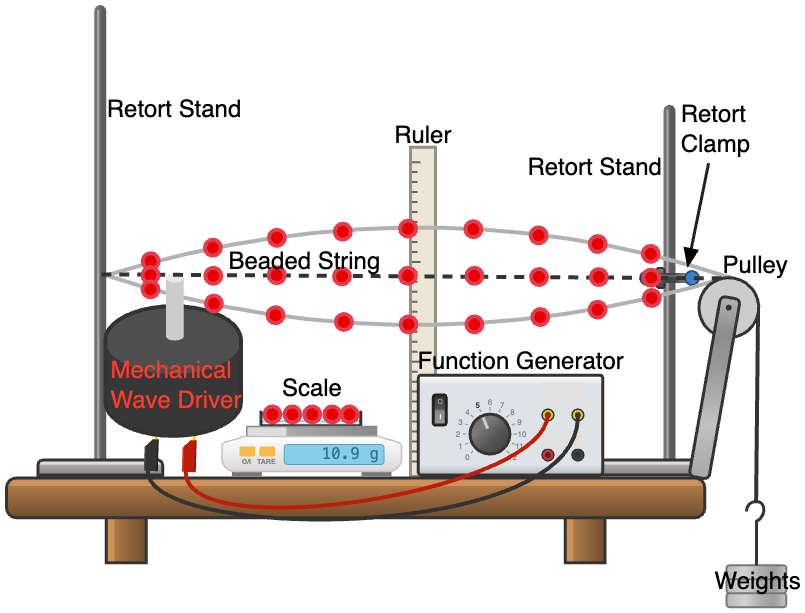
\includegraphics[width=4in]{images/setup.png}
    \caption{The final optics track setup}
    \label{fig:setup}
\end{figure}

\section{Experimental Apparatus}

Materials given were a vertical optics track, a laser diode, rulers, a slide and slide slip, paper, blank track holders, and various lenses. Our setup is illustrated in Figure 1.

% \pagebreak
\section{Procedure}

We setup the optics track with a laser at the top, a blank optics holder in which we placed the slide which we attached a slide cover to by rubbing them together until they stuck and tiny colorful rings could be seen in the glass. We used two lenses to magnify and focus the rings coming out of the slide, which we projected onto paper, and traced the rings cast three times. We also placed a transparent ruler where the slide was to compute the magnification manually instead of doing the magnification computations which could be more error-prone (my eyes are better than my math).

\begin{figure}[ht]
    \centering
    \includegraphics[width=3in]{images/rings.png}
    \caption{The slide looked (exaggeratedly) like this}
    \label{fig:setup}
\end{figure}

\section{Results}

\begin{figure}[ht]
    \centering
    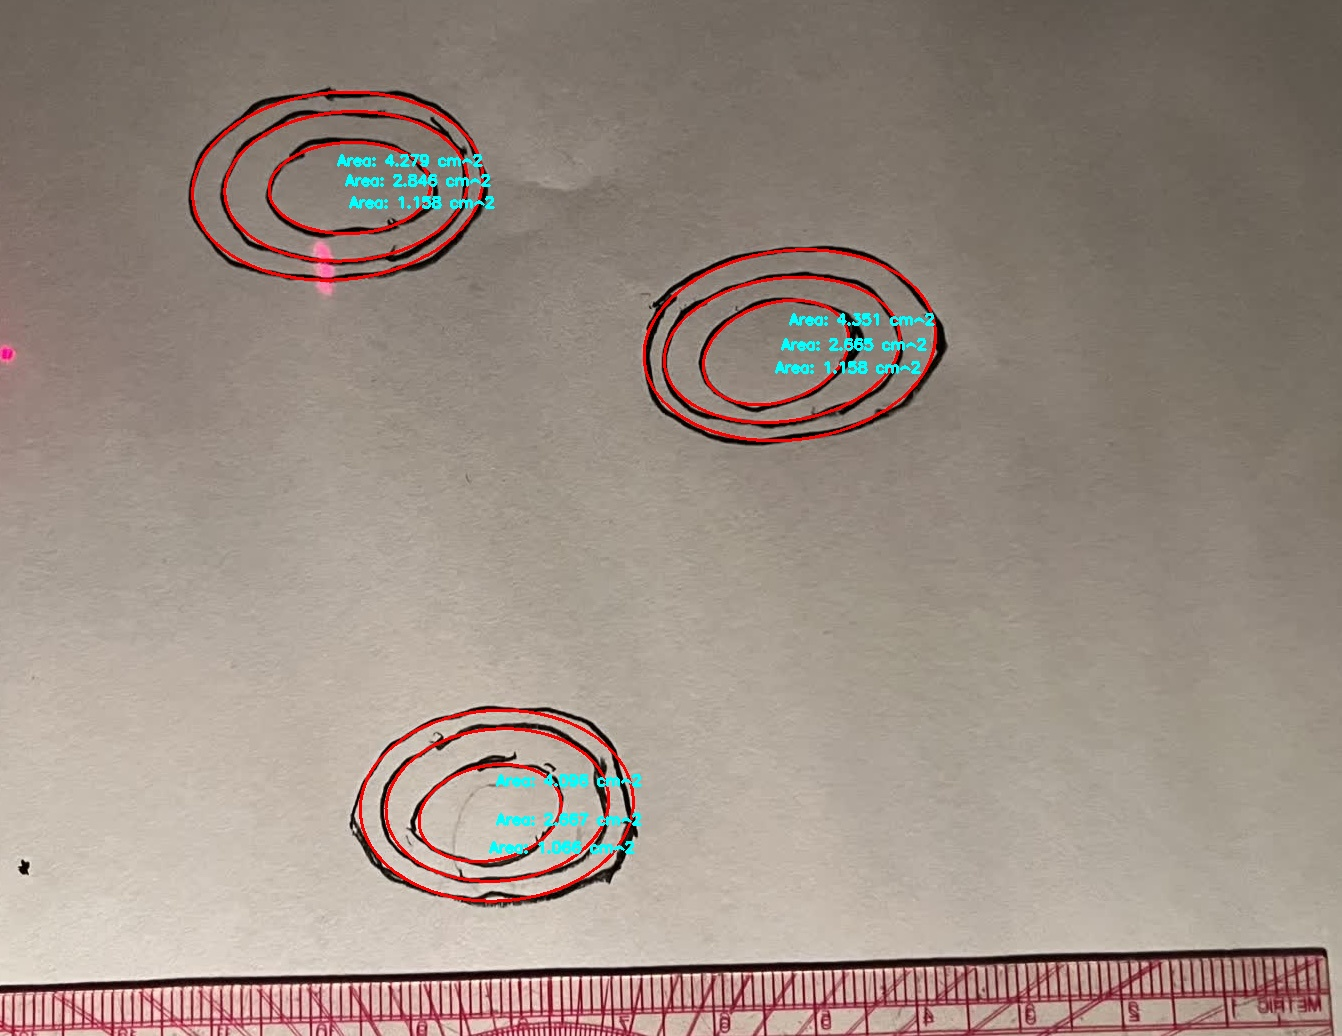
\includegraphics[width=6in]{images/areas.jpg}
    \caption{Measured areas of the traced pattern}
    \label{fig:setup}
\end{figure}

I began by using Python to analyze the areas of our three different sketches of the rings, as shown in Figure 3. However, this was the post-magnification area, so we first have to compute the magnification to get the original area.

As shown in Figure 4, we simply held a transparent ruler in place of the slide, and placed another ruler on the paper we projected onto. We just compared these two measurements to observe a magnification of \textbf{4.3x}.

\begin{figure}[ht]
    \centering
    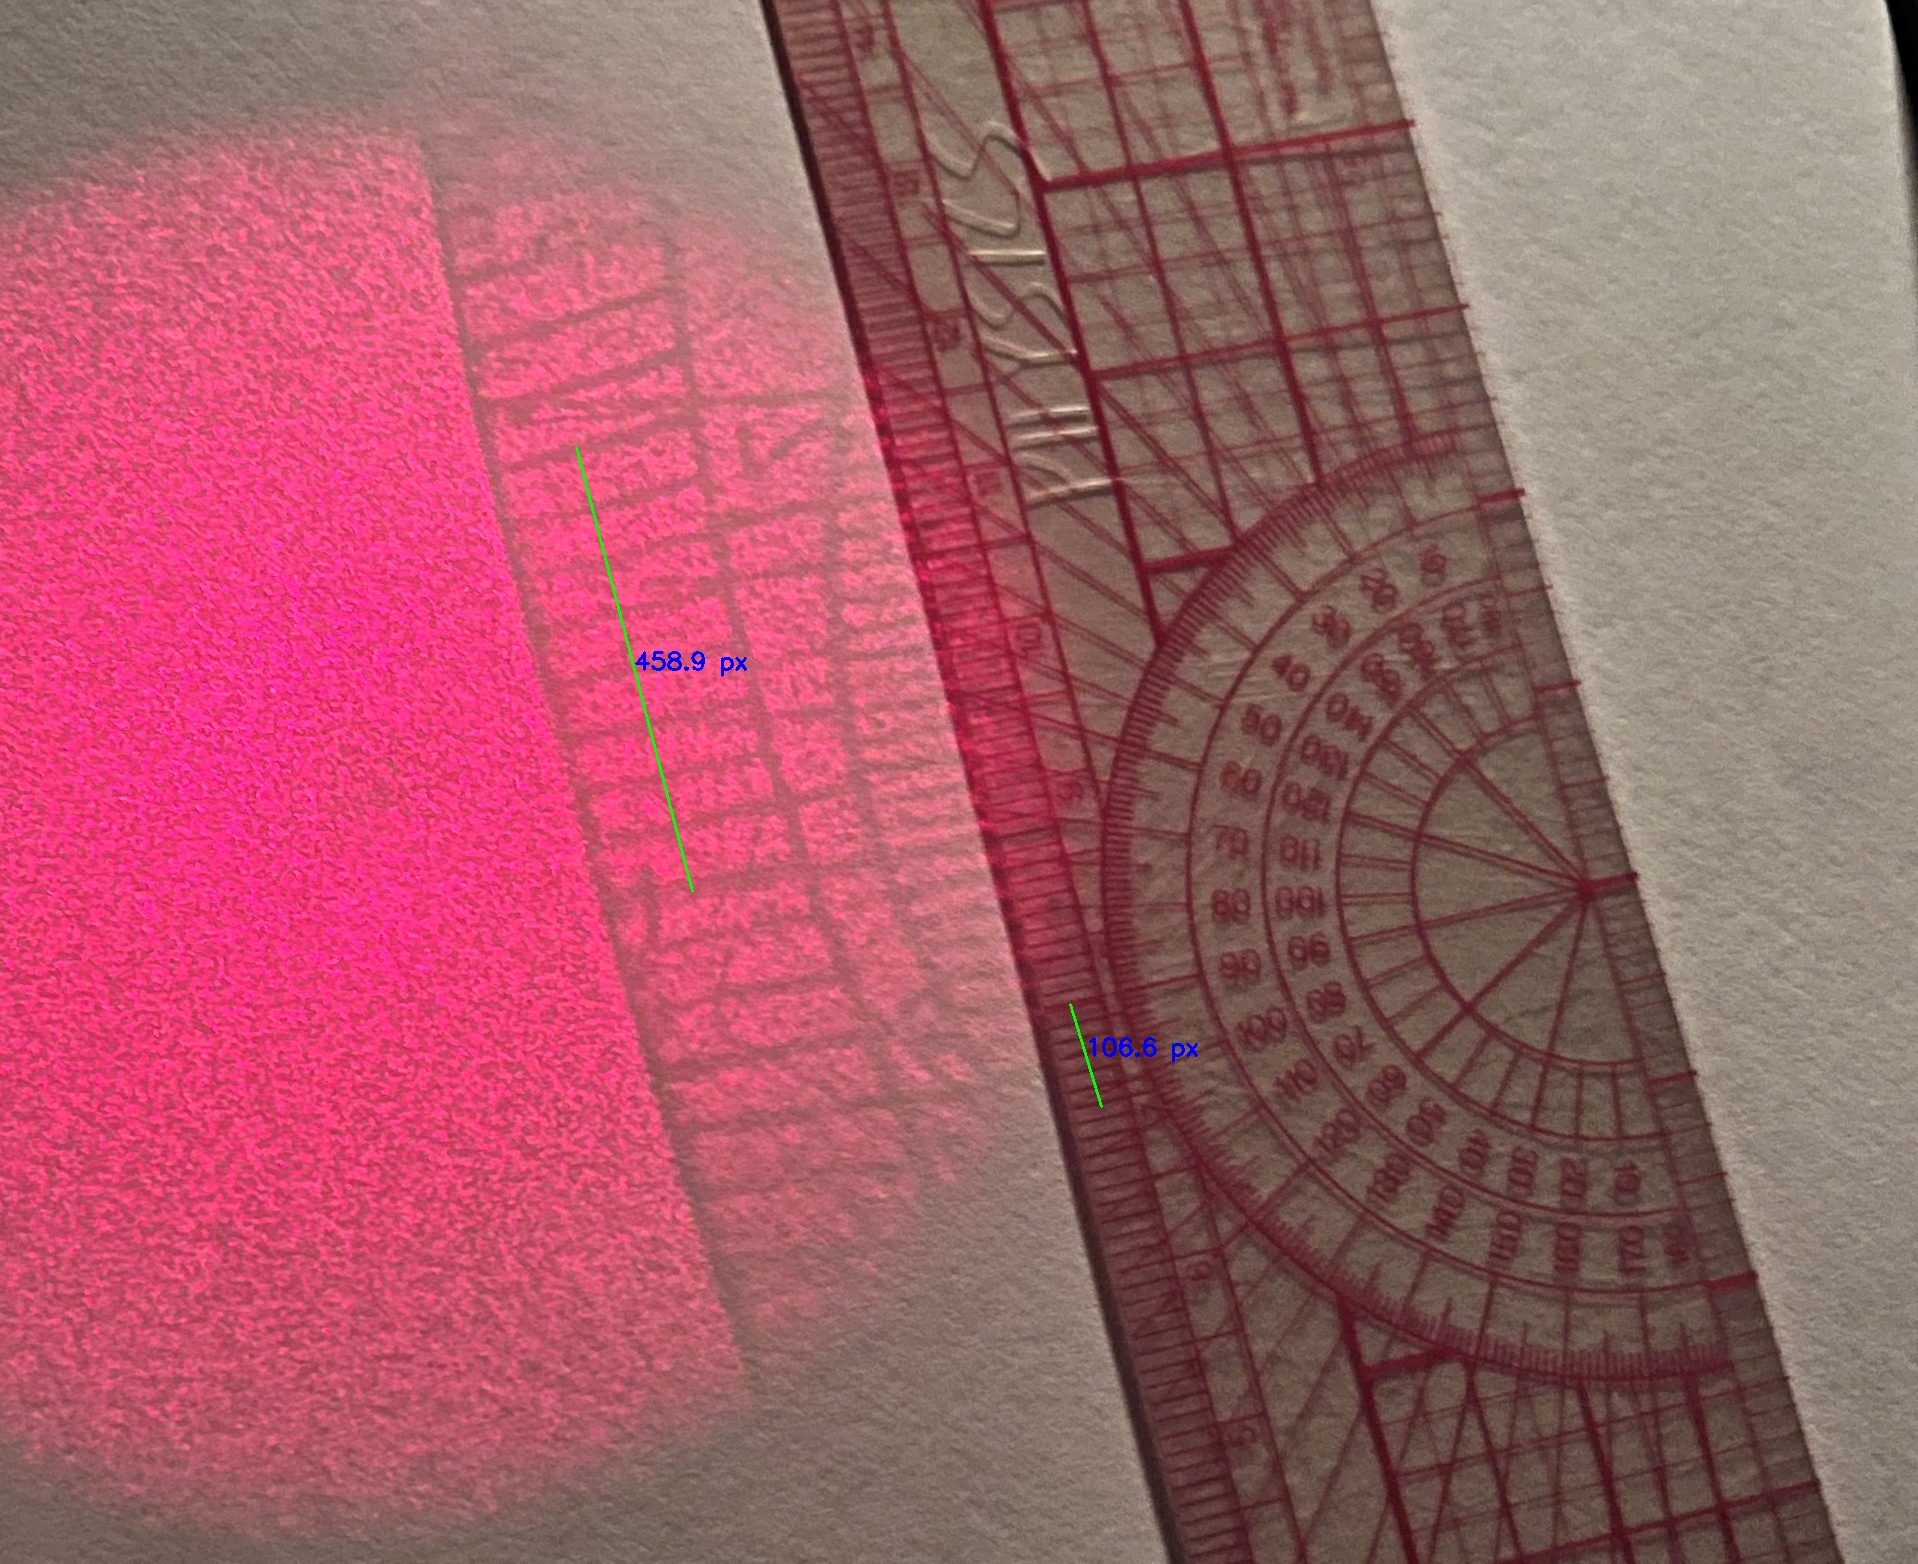
\includegraphics[width=6in]{images/measured_lines.jpg}
    \caption{Measured magnification using rulers}
    \label{fig:setup}
\end{figure}

Finally, to compute the electrostatic force on the slide we use the fact that the shear modulus for Borosilicate glass is 26.3 GPa in the following equation

\begin{equation}
    S=\frac{[\text{shear stress}]}{[\text{shear strain}]}=\frac{\frac{F}{A}}{\frac{x}{\ell}}
\end{equation}

To find $x$, we can use basic geometry on the shape shown in Figure 2. Using our knowledge of interference patterns we can say $r_m^2=\frac{m\lambda R}{n}$ where $n$ is the index of refraction and $m$ is the number of Newton's ring (we'll use $m=1$). So $r^2=\lambda R$, where $R$ is the radius of curvature. While I didn't do the entire derivation, the College of San Mateo has a proof of the fact that $x=\frac{r^2}{2R}$. If we combine these, we get that $x=\frac{\lambda}{2}$.

If we rearrange Equation 1 using this fact, we see that 

\begin{equation}
    F=\frac{SA\lambda}{2\ell}
\end{equation}

We know that the laser is 650 nm and $\ell$ is 150 $\mu$m, and so all the computed results are in Table 1

\begin{table}[h]
\centering
\begin{tabular}{|c|c|c|}
\hline
Ring & Area (cm$^2$) & Force (N) \\
\hline
1 & 0.264 ± 0.001 & 1489.56 ± 1.31 \\
2 & 0.267 ± 0.001 & 1506.59 ± 1.31 \\
3 & 0.247 ± 0.001 & 1388.68 ± 1.31 \\
\hline
\multicolumn{2}{|c|}{Average Force} & $\mathbf{1461.61 \pm 0.44} \textbf{ N}$ \\
\hline
\end{tabular}
\caption{Force Calculations}
\label{tab:force_results}
\end{table}

\section{Conclusions}

We see that the electrostatic force on the slide slip was $\mathbf{1461.61 \pm 0.44} \textbf{ Newtons}$. This seems rather large, but is better than some earlier results of $\approx 10^{17}$ Newtons.

% \bibliographystyle{unsrtnat}
% \bibliography{references}

\end{document}
